\documentclass{article}
\usepackage[hyphens]{url}
\usepackage{mathtools}
\usepackage{amsmath}
\usepackage{listings}
\usepackage{graphicx}
\usepackage[margin=1in]{geometry}
\usepackage{float}
\floatstyle{boxed}
\restylefloat{figure}
\lstset{breaklines=true}
\begin{document}


\title{CS595 Intro to Web Science, Assignment \#5}
\author{Valentina Neblitt-Jones}
\date{October 17, 2013}
\maketitle

The ``friendship paradox'' (\url{http://en.wikipedia.org/wiki/Friendship_paradox})  says that your friends have more friends than you do. \\

\section*{Question 1}

Determine if the friendship paradox holds for your Facebook account. Create a graph of the number of friends (y-axis) and the friends sorted by number of friends (x-axis). (The friends don't need to be labeled on the x-axis.) Do include yourself in the graph and label yourself accordingly. \\

Compute the mean, standard deviation, and median of the number of friends that your friends have. \\

You can download your network in an XML file by using the NameGenWeb Facebook app:  \\

\url{https://apps.facebook.com/namegenweb} \\

You will need to give this app permission to access your Facebook data. Make sure you select "Friend Count" as an Extended Attribute. When you download the data, download it in the GraphML format. \\

If you do not have a Facebook account, email me and I will send you my GraphML file.

\subsection*{Answer to Question 1}

%\begin{itemize}
%\item TMZ.com
%\item Sesame Workshop
%\item VT News
%\item Washington City Paper
%\item Library of Congress 
%\end{itemize}

%Figure \ref{inputfile} showed a sample of the input file. It has the md5 and the URI for each link.

%\begin{figure}[H]
%\centering
%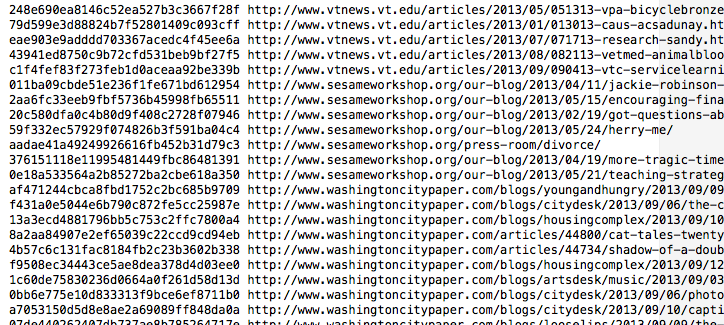
\includegraphics[scale=0.50]{q1/inputfile}
%\caption{Sample of Input File}
%\label{inputfile}
%\end{figure}


\newpage

\section*{Question 2}

Determine if the friendship paradox holds for your Twitter account. Since Twitter is a directed graph, use ``followers'' as value you measure (i.e., ``do your followers have more followers than you?'') \\

Generate the same graph as in question \#1, and calculate the same mean, standard deviation, and median values. \\

For the Twitter 1.1 API to help gather this data, see: \\

\url{https://dev.twitter.com/docs/api/1.1/get/followers/list} \\

If you do not have followers on Twitter (or don't have more than 20), then use my Twitter account ``phonedude\_mln''.

%\begin{table}[!h]
%\centering
%\caption{10 Hits for the term ``shadow'', ranked by TFIDF}
%\begin{tabular}{c c c c}
%\hline
%TFIDF & TF & IDF & URI \\
%\hline
%\hline
%0.150 & 0.014 & 10.680 & http://foo.com \\
%0.085 & 0.008 & 10.680 & http://bar.com \\
%\hline
%\end{tabular}
%\end{table}

\subsection*{Answer to Question 2}


\clearpage

\section*{Extra Credit - LinkedIn (2 points)}

Repeat question \#1, but with your LinkedIn profile.

\subsection*{Answer to Extra Credit - LinkedIn}

\clearpage

\section*{Extra Credit - Twitter (1 point)}

Repeat question \#2, but change ``followers'' to ``following''? In other words, are the people I am following following more people?

\subsection*{Answer to Extra Credit - Twitter}

\end{document}